\documentclass{article}
\usepackage{float}
\usepackage{array}
\newcolumntype{P}[1]{>{\RaggedRight\arraybackslash}p{#1}}
\newcolumntype{M}[1]{>{\RaggedRight\arraybackslash}m{#1}}
\usepackage{amsmath}
\usepackage{mathtools}
\usepackage{amssymb}
\newcommand{\tarc}{\mbox{\large$\frown$}}
\newcommand{\arc}[1]{\stackrel{\tarc}{#1}}
\usepackage{setspace}
\usepackage{graphicx}
\usepackage{wrapfig}
\usepackage[export]{adjustbox}
\usepackage{geometry}\geometry{left=10mm,right=10mm,top=10mm,bottom=20mm}
\usepackage{xepersian}
\usepackage{mathspec}
\usepackage{enumerate}

\settextfont[Scale=1.2]{XB Niloofar.ttf}
\setdigitfont{XB Niloofar.ttf}

\begin{document}

\onehalfspacing
\large
	\begin{center}
		\small به نام او\\ 
		\vspace*{6pt}
		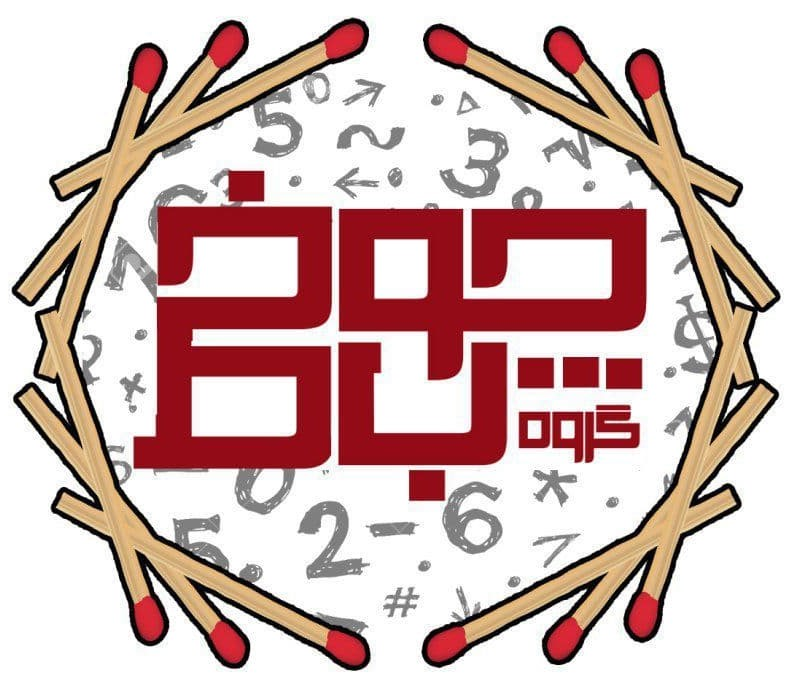
\includegraphics[scale=0.2]{Choobkhat_Logo.jpg}
	\end{center}
	\begin{small}
		گروه آموزشی چوب‌خط
		\vspace*{-.01cm}\hfill 12 فروردین 1399 \\
		آزمون آزمایشی المپیاد کامپیوتر 
		\vspace*{-.01cm}\hfill زمان : 135 دقیقه \
	\end{small}
	\begin{center}
		\begin{large}
		آزمون پاسخ‌کوتاه المپیاد کامپیوتر
		\end{large}
	\end{center}
	\begin{center}
		\hrule width 1\textwidth
	\end{center}
	\begin{enumerate}
	%////////////////////////////////////////////////1
    \item    
  به چند طریق میتوان 7 خانه‌ی باقی مانده از جدول زیر را با اعداد طبیعی پر کرد به طوری که هر عدد بر اعداد بالا و چپش (در صورت وجود) بخش پذیرباشد؟\\
   \begin{figure}[H]
   	\centering
   	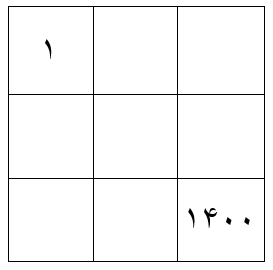
\includegraphics[scale=0.4]{P1.png}
   \end{figure}
    %////////////////////////////////////////////////2
		\item  
هیکاپ به لانه ی اژدهاها رفته و در مختصات $(1,1)$ قرار دارد. به خاطر تعداد زیاد اژدهاهای غیر اهلی، پشم‌هایش فر خورده است و هر ثانیه به طور تصادفی به یکی از خانه های مجاور میرود. (بالا پایین چپ راست). میدانیم در خانه هایی با مختصات $(6i, 6j)$ یک اژدهای عصبانی، و در خانه هایی با مختصات $(6i+3, 6j+3)$ پناهگاه وجود دارد. احتمال اینکه هیکاپ از این ماجرا جان سالم به در ببرد چه قدر است؟
\\
\\
    %////////////////////////////////////////////////3
    \item
چند جایگشت از اعداد 1 تا 8 مانند $a_1, a_2, \cdots , a_8$ وجود دارد به طوری که: 
$ a_1 - a_2 + a_3 - a_4 + a_5 - a_6 + a_7 - a_8 = 0 $
 \\
    %////////////////////////////////////////////////4
		\item
		در دریای سالِن 9 جزیره وجود دارد که توسط تعدادی جاده هوایی به یکدیگر متصل اند. 3 تا از جاده‌ها یک طرفه شده اند و می‌خواهیم بقیه‌ی جاده ها رانیز طوری یک طرفه کنیم که از هیچ شهری نتوان با گذر از تعدادی جاده به خودش بازگشت. این کار به چند طریق ممکن است؟\\
		\begin{figure}[H]
			\centering
			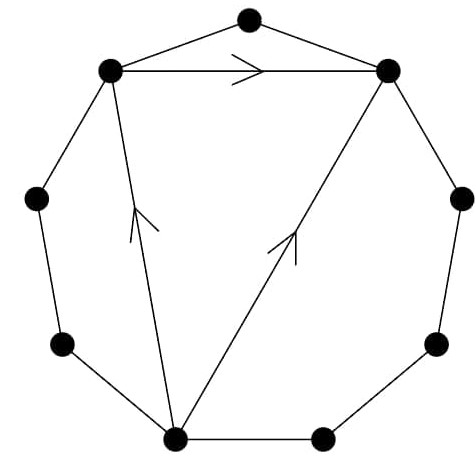
\includegraphics[scale=0.3]{P5.jpg}
		\end{figure}
    %////////////////////////////////////////////////5
    \item
ماتریس 3×2 ای را میخواهیم با اعداد 0و 1و 2 پر کنیم به طوری که جمع اعداد هر سطر و هر ستون مضرب 3 باشد. این کار به چند حالت ممکن است؟\\
\\
    %////////////////////////////////////////////////6
    \noindent
    
		\item 
نرگس به رافنات و تافنات گفت که بستنی فروشی باز کرده و آنها قبول کردند که فردا به آنجا بروند و بستنی بخرند. امشب نرگس باید تعدادی بستنی با وزن طبیعی درست کند و فردا که آنها آمدند هر کدام مقداری بستنی سفارش می‌دهند. (رافنات $p$ کیلو و تافنات $q$ کیلو) نرگس باید بتواند تعدادی بستنی را روی هم چیده، بستنی درخواست شده‌ی هر کدام را بدهد. نرگس امشب حداقل چند بستنی باید درست کند؟ (رافنات و تافنات برای اینکه به نرگس فشار مالی وارد نشود طوری سفارش می‌دهند که 
$p + q < 1400$
.
 توجه کنید که نرگس از اعداد $p$ و $q$ خبر ندارد.)\\
 \\
    %////////////////////////////////////////////////7
    	\item 
می‌دانیم دقیقا یک نفر از ۳ اژدهاسوار(فیشلگز، اسناتلات و تافنات) نان‌خامه‌ای آسترید را دزدیده اند. هر اژدهاسوار فقط یکی از این سه نفر را نام میبرد و می‌گوید دزد است یا بیگناه. (اژدهاسواران می‌توانند جملات یکسان بگویند) بعد از شنیدن حرف‌های اژدهاسواران با دانستن اینکه دقیقا یک نفر دروغ می‌گوید، آسترید در چند حالت از صحبت های سه اژدهاسوار می‌تواند دزد را پیدا کند؟ (توجه کنید که فرد دروغگو لزوما همان دزد نیست)\\
\\
    %////////////////////////////////////////////////8
    \item
بی‌دندون و هیکاپ با هم بازی می‌کنند. یک جدول $ 8\times 8$ دارند. ابتدا بی‌دندون عدد صحیح مثبت $k$ را انتخاب و در $k$ خانه‌ی دلخواهش از جدول حرف $B$ را می‌نویسد. سپس هیکاپ $k+1$ خانه از جدول را انتخاب میکند و در آنها حرف $H$ را می‌نویسد. اگر در در سه خانه متوالی جدول (چه افقی چه عمودی) به ترتیب حروف "$"B B H"$" یا حروف "$"H B B"$" وجود داشت بی‌دندون میبرد، در غیر این صورت هیکاپ برنده است. کمترین مقدار $k$ را بیابید که بی‌دندون با انتخاب آن استراتژی برد دارد.\\
\\
    %////////////////////////////////////////////////9
    \item
بی دندون دارد در یک صفحه مختصات بازی میکند. با شروع از خانه‌ی $(0,0) $در هر گام او میتواند یک واحد به بالا یا یک واحد به راست بپرد. خانه‌هایی با مختصات $(2k+1, 2k’+1)$ مسدود اند و بی‌دندون نمیتواند به آنها برود. او به چند طریق میتواند به خانه‌ی $(8,14)$ برسد؟
	\end{enumerate}
\end{document}
